\documentclass{article}

% Language setting
% Replace `english' with e.g. `spanish' to change the document language
\usepackage[portuguese]{babel}

% Set page size and margins
% Replace `letterpaper' with `a4paper' for UK/EU standard size
\usepackage[a4paper,top=2cm,bottom=2cm,left=3cm,right=3cm,marginparwidth=1.75cm]{geometry}

% Useful packages
\usepackage{amsmath}
\usepackage{graphicx}
\usepackage[colorlinks=true, allcolors=blue]{hyperref}
\usepackage{csvsimple}
\usepackage{svg}

\title{Relatório da Tarefa 4 - Rede Neural}
\author{Manoel Marcelo da Silva\\
Instituto de Computação -- Universidade Federal do Rio de Janeiro\\
manoelms@ic.ufrj.br
}

\begin{document}
\maketitle

\section{Introdução}

O objetivo dessa tarefa é analisar e estudar as redes neurais, como o Multi-Layer Perceptron Classifier, em um dataset simples, neste caso o IRIS. Como veremos a seguir, apesar de ser um modelo extremamente poderoso e simples de ser aplicado, ainda mais que estamos usando a biblioteca sci-kit learn no Python, ele é bastante seletivo em relação a alguns tipos de parâmetros e por isso precisa ter um cuidado a mais.

\section{Dataset}

\subsection{Iris Dataset}

Usaremos o Iris dataset, encontrado livremente em sites como o \href{https://www.kaggle.com/datasets/uciml/iris}{Kaggle} e no próprio \href{https://scikit-learn.org/stable/auto_examples/datasets/plot_iris_dataset.html}{Sci-kit Learn}. Este dataset com 150 instâncias possui 4 atributos numéricos e um categórico, sendo eles, respectivamente: 

\begin{itemize}
    \item sepalLengthInCM 
    \item sepalWidthInCM	 
    \item petalLengthInCM	
    \item petalWidthInCM	
    \item target - Com 3 diferentes tipos de Iris (Setosa, Versicolour, and Virginica)
\end{itemize}

\subsection{Pré-Processamento}
Como o Multi-Layer Perceptron é muito sensível ao dimensionamento do atributo (feature scaling), é ideal que os atributos numéricos estejam normalizados. Assim, foi usado o StandardScaler, da própria biblioteca Sci-kit Learn, nesses atributos.

\subsection{Separando o dataset}
O dataset foi separado previamente em $ 80\% $  para treino e $ 20\% $ para teste para ser usado posteriormente após a seleção da arquitetura da rede neural. Além disso, foi usado o modo estratificado, para manter a mesma proporção das classes.

\section{Arquiteturas neurais}

Para selecionar a arquitetura ideal para a rede neural foram testados diversos parâmetros do MLPClassifier. Para isso, foi feito um K-Fold Estratificado de tamanho 5 em relação à divisão feita anteriormente, com a mesma proporção de classes para manter a consistência no treino.

\subsection{Tamanho das camadas escondidas e iterações máximas}
Após vários testes, foi constatado que com um número grande o suficiente de neurônios, com determinado número de camadas, qualquer um dos 3 tipos de funções de ativação (ReLU, Tanh, Logistic) chegam à uma classificação aceitável com mais de 95\% de acurácia. Porém, com um número mínimo de 10 neurônios em uma camada é possível conseguir tal acurácia com menos processamento, sendo este o número escolhido. Além disso, foi limitado para no máximo 1000 iterações do gradiente descendente. 


\subsection{Logistic}

Usando a função de ativação logística temos os seguintes resultados na função de perda em diferentes k folds estratificados:

\begin{figure}[ht!]
    \centering
    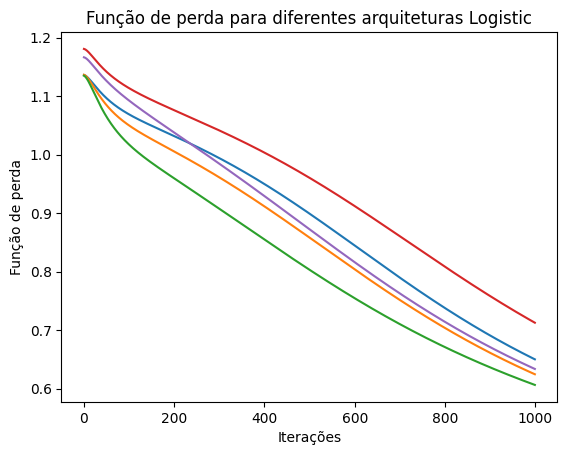
\includegraphics[width=0.5\linewidth]{logistic_loss.png}
    \caption{Função de Perda - Logistic}
    \label{fig:enter-label}
\end{figure}

Sua acurácia de teste é, em média, de apenas $80\%$. Porém, com mais neurônios fica bem melhor (50 - 97\%), ao custo de performance.

\subsection{Tanh}

Já usando a função de ativação Tanh temos os seguintes resultados na função de perda em diferentes k folds estratificados:

\begin{figure}[ht!]
    \centering
    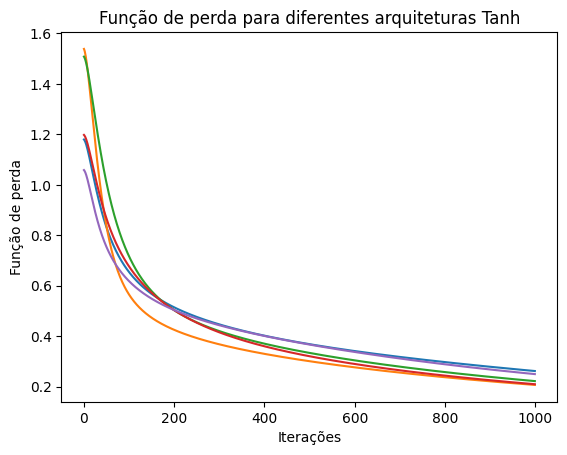
\includegraphics[width=0.5\linewidth]{tanh_loss.png}
    \caption{Função de Perda - Tanh}
    \label{fig:enter-label}
\end{figure}

Sua acurácia de teste é aproximadamente $97\%$, sendo um ótimo candidato para escolha.

\subsection{ReLU}

Por fim, usando a função de ativação ReLU, padrão do Sci-Kit, temos os seguintes resultados na função de perda em diferentes k folds estratificados:

\begin{figure}[ht!]
    \centering
    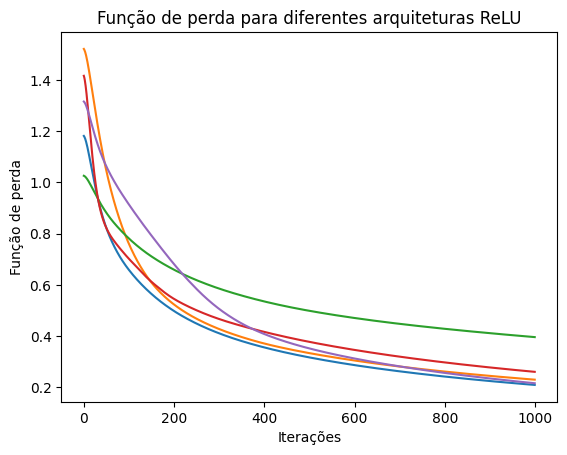
\includegraphics[width=0.5\linewidth]{relu_loss.png}
    \caption{Função de Perda - ReLU}
    \label{fig:enter-label}
\end{figure}

Similar ao Tanh, sua acurácia de teste é, em média, $97\%$, sendo também uma ótima escolha.

\subsection{Conclusão}
Após fazer vários testes, foi constatado que a função logística pode funcionar, mas comparado as outras opções não parece bom, já que para ter uma acurácia interessante é necessário muitos neurônios, ou seja, mais custoso. Observando a sua função de perda, é perceptível sua linearidade, o que não é um bom sinal em comparação com as outras opções, que é quase logarítmica.

Já o ReLU e o Tanh são bem eficientes e possuem uma ótima acurácia, ambas as escolhas são boas. No entanto, iremos escolher o Tanh pois ela é um pouquinho melhor em relação ao ReLU, como vemos no gráfico abaixo.
\begin{figure}[ht!]
    \centering
    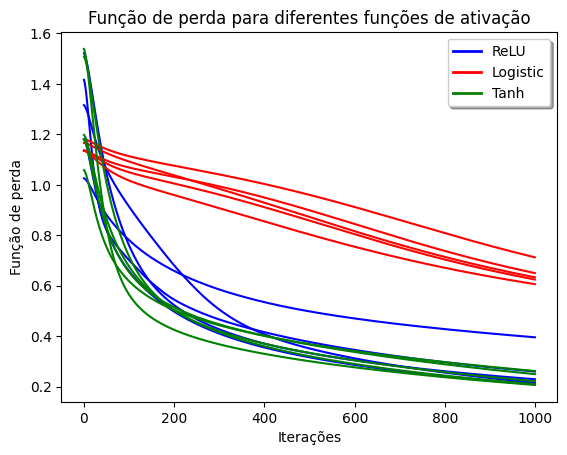
\includegraphics[width=0.5\linewidth]{diff_loss.png}
    \caption{Todas as funções}
    \label{fig:enter-label}
\end{figure}

\newpage
\section{Resultados}

Por fim, a rede neural possui 4 neurônios de entrada, 10 neurônios na camada escondida e 3 de saída. Sua função de ativação é a Tanh.

\begin{figure}[ht!]
    \centering
    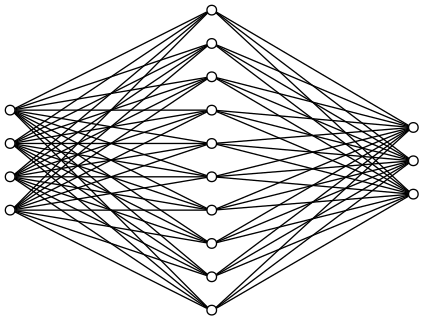
\includegraphics[width=0.5\linewidth]{iris.png}
    \caption{Rede Neural final}
\end{figure}

Ao testar com os 20\% do dataset separados anteriormente, temos a seguinte matriz de confusão:

\begin{figure}[ht!]
    \centering
    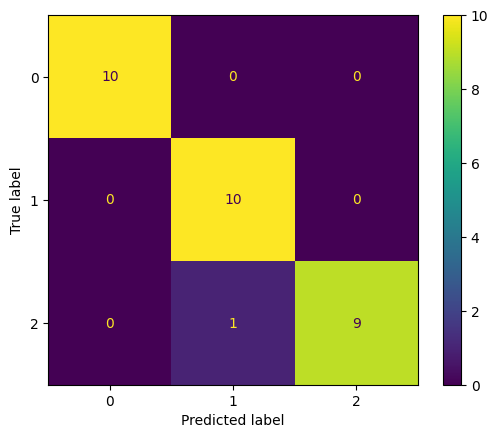
\includegraphics[width=0.5\linewidth]{final_conf.png}
    \caption{Matriz de Confusão}
\end{figure}

E a seguinte função de perda:

\begin{figure}[ht!]
    \centering
    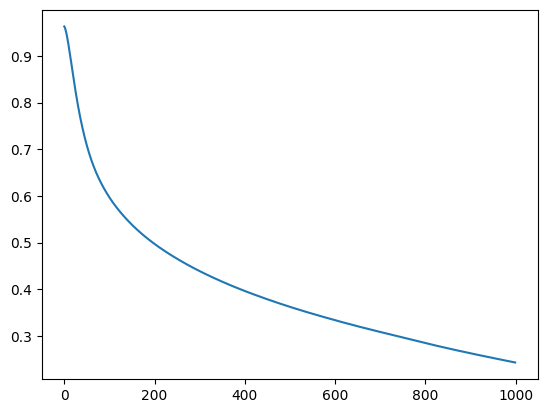
\includegraphics[width=0.5\linewidth]{final_loss.png}
    \caption{Função de perda final}
\end{figure}


\end{document}